\chapter{Introduction}
\label{chap-1-intro}
\begin{ChapAbstract}
In this chapter, ...
\end{ChapAbstract}


\section{Overview} % 1 page

\section{Introduction to Remote Sensing} % 2 pages

Remote sensing imagery is the data that acquired from satellites on the sky. The uses of those data might be making surface map (for examples: Google Maps, Apple Map); creating maps of land surface temperature, reflectance and elevation; monitoring hydrology and land changes, etc. 


There are many kinds of satellites. In this report, I will only focus on 2 types: optical-type and radar-type.

\subsection{Optical satellites}

Satellites with optical sensors provide images of the Earth over relatively large areas and are useful in the production of hydrology and vegetation maps. The sensors function in the optical part of wavelength spectrum, including visible, near infrared and short-wave infrared wavelengths. Satellite sensors commonly used for detailed mapping include Landsat, Sentinel-2, etc., with moderate resolution (resolution is approximately from 10 to 30 meters).
\begin{figure}
	\centering
	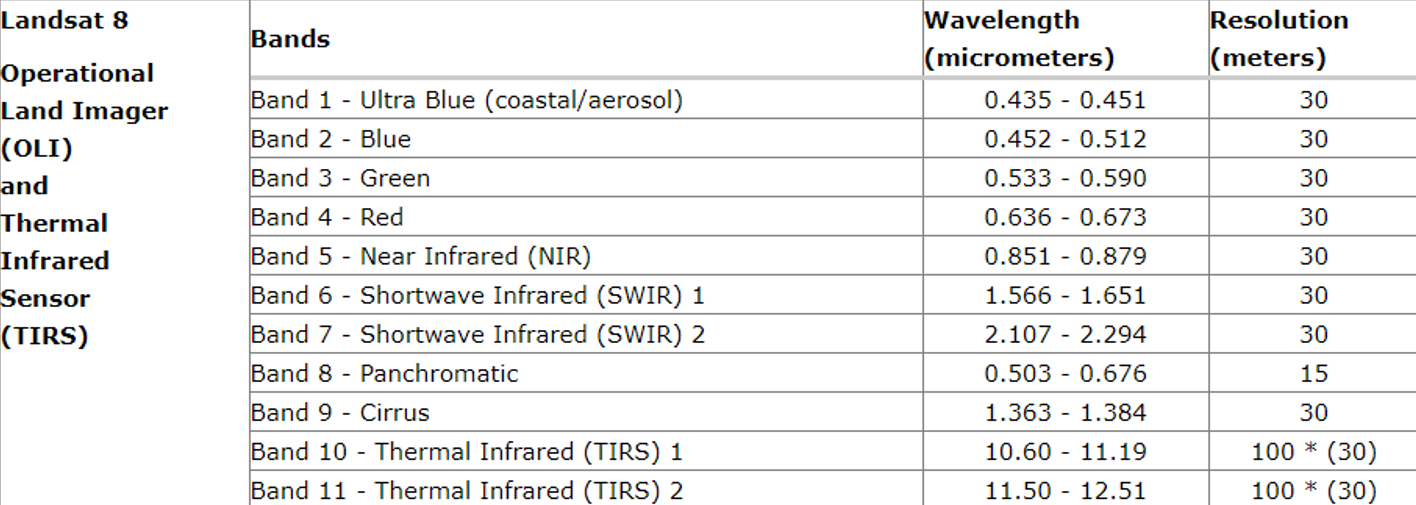
\includegraphics[width=0.8\textwidth]{figures/wavelengthL8.png}
	\caption{Landsat 8 data specification. Source: USGS}
\end{figure}
Wavelengths of optical satellites are useful for distinguishing between forest types and other vegetation classes. Optical satellite data can be combined with laser data because the color information in optical satellite data can distinguish different vegetation types while laser data provides additional information about terrain or vegetation characteristics. 
\begin{figure}
	\begin{subfigure}{0.24\textwidth}
		\centering
		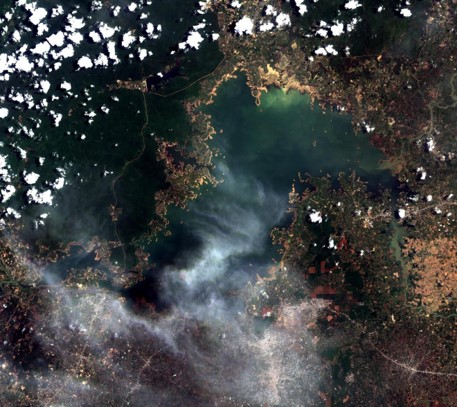
\includegraphics[width=.8\linewidth]{figures/trueColor.jpg}
		\caption{}
	\end{subfigure}
	\begin{subfigure}{0.24\textwidth}
		\centering
		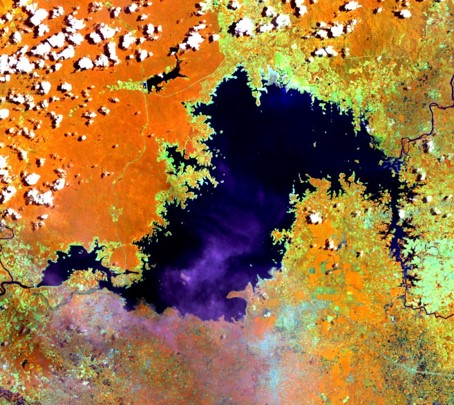
\includegraphics[width=.8\linewidth]{figures/landwater.jpg}
		\caption{}
	\end{subfigure}
	\begin{subfigure}{0.24\textwidth}
		\centering
		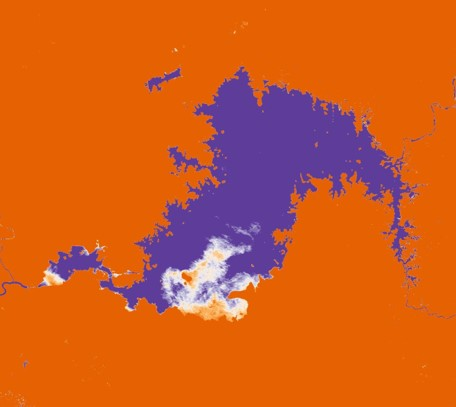
\includegraphics[width=.8\linewidth]{figures/ndwi.jpg}
		\caption{}
	\end{subfigure}
	\begin{subfigure}{0.24\textwidth}
		\centering
		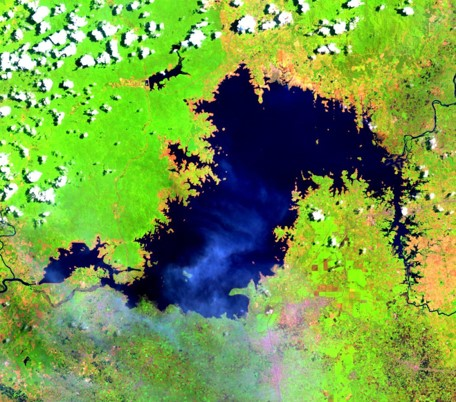
\includegraphics[width=.8\linewidth]{figures/agriculture.jpg}
		\caption{}
	\end{subfigure}
	\centering
	\caption{Samples of bands combinations from Landsat 8 data files.
		\textbf{(a)} True Color (B4, B3, B2).
		\textbf{(b)} Land/Water (B5, B6, B4).
		\textbf{(c)} Normalized difference water index(B3 - B5)(B3 + B5).
		\textbf{(d)} Agriculture(B6, B5, B2)}
\end{figure}

\subparagraph{The Landsat 8 Pre-Collection Quality Assessment (QA) band}
QA band is a part of Landsat 8 data files. Each pixel in the QA band contains integer that represent bit-packed combination of surface, atmosphere and sensor conditions that can affect overall usefulness of a given pixel. Depending on its pixel value (mostly depending on QA Bits), we can detect that pixel is a snow/ice, cloud or water (because these are mainly formed by water) or detect the cloud direction due to cirrus confidence. For more information about QA Band, see at: \href{https://landsat.usgs.gov/qualityband}{https://landsat.usgs.gov/qualityband}.

\begin{figure}
	\centering
	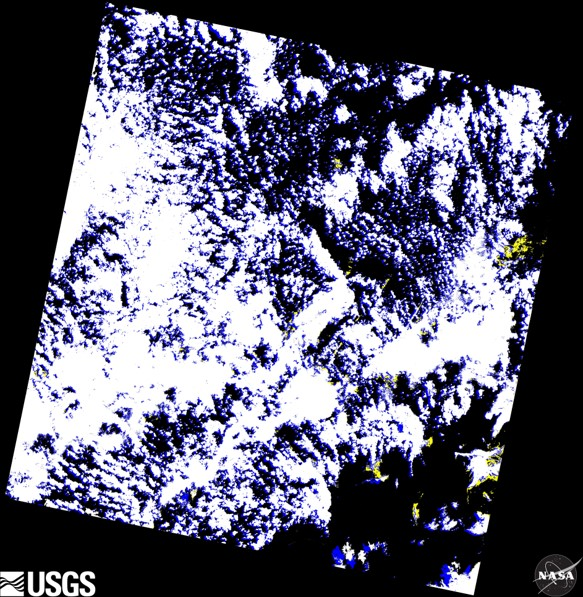
\includegraphics[width=0.32\textwidth]{figures/qaL8.jpg}
	\caption{Landsat 8 QA Band, Tri An Reservoir. Date taken: May 30, 2017}
\end{figure}

\subsection{Radar satellites}

Radar satellites can solve problem of satellites image on cloud days, and this is the biggest advantage of radar data over optical data. They are not affected by cloud because of its instrument specifications. For example, Sentinel-1 satellites use the C-Band Synthetic Aperture Radar (SAR). This colored Sentinel-1 SAR image is produced by showing the two polarisations (VV and VH i.e. vertical polarisation send for the radar signal and vertical or horizontal receive). 

\begin{figure}[h!]
	\centering
	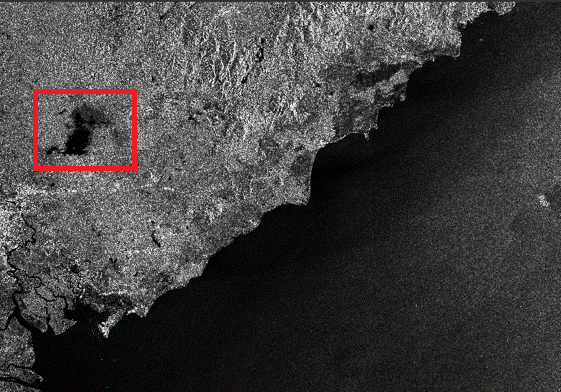
\includegraphics[width=0.8\textwidth]{figures/sarImgVVS1.png}
	\caption{Sentinel-1 (band VV) image, Tri An Reservoir. Date taken: June 11, 2017}
\end{figure}	

For this advantage, it can be used for evaluating my proposed methods on water body that segmented from the recovered image of optical satellites.

\section{Related Work} % 2 pages

\section{Contributions and Outlines} % 1 pages

